\documentclass{article}
\usepackage[utf8]{inputenc}
\usepackage[margin=2cm]{geometry}
%\usepackage{enumitem}

% maths packages
\usepackage{amsmath}
\usepackage{amssymb}
\usepackage{amsthm}

% graphics packages
\usepackage{graphicx}
%\usepackage{subfig}
\usepackage{tikz}
\usetikzlibrary{positioning, circuits.logic.US}

\title{Quantum Bernoulli Factory}
\author{Suzie Brown}
\date{\today}

% bibliography
\usepackage[round, sort&compress]{natbib}
\usepackage{har2nat} %%% Harvard reference style
\bibliographystyle{agsm}

% theorems
\newtheorem{thm}{Theorem}
\theoremstyle{definition}
\newtheorem{defn}{Definition}
\newtheorem{example}{Example}

% probability symbols
\newcommand{\PR}{\mathbb{P}}
\newcommand{\E}{\mathbb{E}}
\newcommand{\V}{\operatorname{Var}}
\newcommand{\iidsim}{\overset{iid}{\sim}}
\newcommand{\eqdist}{\overset{d}{=}}

% distributions
\newcommand{\Bern}{\operatorname{Bernoulli}}
\newcommand{\Geom}{\operatorname{Geom}}

% project-specific commands
\newcommand{\A}{\mathcal{A}}

%% IBM's actual quantum computer you can experiment on:
% https://quantumexperience.ng.bluemix.net/qx/experience

\begin{document}
\maketitle
\section*{Bernoulli factories}
Suppose we have access to a black box producing coin flips where the probability of observing heads is $p$. Roughly speaking, a Bernoulli factory is an algorithm that uses queries of this black box to produce a coin flip where the probability of observing heads is $f(p)$, for some specified function $f$.

Let us now make this notion more precise.
\begin{defn}\label{defn:bern_fact}
Let $f: S\to[0,1]$ be a function with domain $S \subseteq [0,1]$, and suppose we have a sequence of Bernoulli random variables $X_1,X_2,\dots \iidsim \Bern(p)$ with unknown parameter $p \in [0,1]$. 
Let $U \in \mathcal{U}$ denote a set of auxiliary random variables with known distributions, independent of $p$. Let $\tau$ be a stopping time with respect to the natural filtration, such that $\PR(\tau<\infty)=1$.
% , and let $T:=\sup_{U,\mathbf{X}} \tau$.
A \emph{Bernoulli factory} is a function $\A : \mathcal{U} \times \{0,1\}^T \to\{0,1\}$ such that $\A(U,X_1,\dots,X_T) \sim \Bern(f(p))$ for all $p \in [0,1]$. For brevity we also denote $Y := \A(U,X_1,\dots,X_T)$.
% for all U?
\end{defn}
% define T ???
% Just sort out this definition...
% this is a special case of the `simulability' definition given in Keane1994.
% obviously must restrict to p \in (0,1) for sensible cases. ?

% Define simulable and strongly simulable
% Remark that any constant function (i.e. indep of p) is simulable, but not nec. strongly.

\begin{example}\label{ex:bf_half}
$f(p) \equiv 1/2$.\\
The following solution to this problem is described in \citet{vonneumann1951}.
We flip the coin twice and, if the two outcomes are different, take the second one as the result. If the outcomes are the same, we start again.
In this case no auxiliary random variable $U$ is required.
\begin{align*}
& \tau = \min\{ t \in \{2,4,\dots\} : X_{t-1} \neq X_t \} \\
& \A(X_1,\dots,X_T) = X_\tau
\end{align*}
It is easy to show that this procedure produces heads with probability 1/2:
\begin{equation*}
\PR(Y=1) = \PR(X_\tau = 1) = \PR(X_2 = 1 \mid X_2\neq X_1) = \frac{\PR(X_1 = 0, X_2 = 1)}{\PR(X_1 = 0, X_2 = 1) + \PR(X_1 = 1, X_2 = 0)} = \frac{p(1-p)}{2p(1-p)} = \frac{1}{2}
\end{equation*}
The running time $\tau$ of this Bernoulli factory is random and unbounded. In particular, 
$\tau \eqdist 2\times\Geom(2p(1-p))$. The running time is minimised when $p=1/2$ (i.e.\ we already have a fair coin), in which case the expected running time is $\E(\tau)=4$. This is why \citet{vonneumann1951} claims ``the amended process is at most 25 percent as efficient as ordinary coin-tossing''. He motivates this as a technique to ensure perfectly unbiased coin flips, although the more biased the original coin flipping procedure, the less efficient this correction will be, as illustrated in Figure \ref{fig:vonneumann_runtime}.
\begin{figure}
\centering
\includegraphics[width=0.8\textwidth]{vonneu_runtime.pdf}
\caption{Expected running time of Von Neumann's $f(p)=1/2$ procedure. When $p$ is not too far from 1/2, the running time is moderate, but as $p$ gets close to 0 or 1 the running time grows unboundedly. The expected running time achieves its minimum of four queries when $p=1/2$.}\label{fig:vonneumann_runtime}
\end{figure}
\end{example}

\begin{example}\label{ex:bf_pk}
$f(p) = p^k, k\in\{1,2,\dots\}$.\\
This problem is solved easily by flipping the coin $k$ times and outputting heads only if all $k$ flips return heads. Again no auxiliary random variable is required.
\begin{align*}
& \tau = k \\
& \A(X_1,\dots,X_T) = \mathbb{I}\{X_1 =1, X_2=1 ,\dots,X_\tau=1\}
\end{align*}
In this case the running time is deterministically equal to $k$. It is clear that this procedure produces heads with probability $p^k$, since 
\begin{equation*}
\PR(Y=1) = \PR(X_1 = 1, \dots, X_k = 1) = \PR(X_1 = 1)\dots \PR(X_k = 1) = \PR(X_1 = 1)^k = p^k
\end{equation*}
The procedure can be sped up if we allow a random running time, still bounded above by $k$, by stopping the process early if tails comes up (in which case we know immediately that the output will be tails). In this case we have
\begin{equation*}
\tau = k \wedge \min\{t \in \{1,2,\dots\}:X_t=0 \}
\end{equation*}
and $\tau \eqdist \min\{k, \Geom(1-p)\}$.
Figure \ref{fig:p2_runtime} shows the expected running time of this procedure for a few values of $k$. We see that early stopping can significantly reduce the expected running time when $p$ is not close to 1, and that the gain in efficiency is greater for larger $k$. In the case $k=1$, where $f$ is the identity, the number of coin flips required is deterministically equal to one, for any $p$.
\begin{figure}
\centering
\includegraphics[width=0.8\textwidth]{pk_runtime.pdf}
\caption{Expected running time for the $f(p)=p^k$ Bernoulli factory described, with early stopping. Without early stopping, the running time is deterministically equal to $k$. The early stopping procedure significantly increases the efficiency, particularly when $p$ is small or $k$ is large. The minimum number of queries is one for all $k$ and $p$, and of course the $k=1$ (identity) Bernoulli factory requires exactly one query for any $p$.}\label{fig:p2_runtime}
\end{figure}
\end{example}

A natural extension of Example \ref{ex:bf_pk} is that products of simulable functions are themselves simulable. That is, given a Bernoulli factory for $f(p)$ and another for $g(p)$, it is possible to produce a Bernoulli factory for $f(p)g(p)$, by performing the two procedures one after the other and returning heads only if both return heads.
As long as the procedures for $f$ and $g$ finish in finite time almost surely, then so will the $f g$ procedure, and if the $f$ and $g$ procedures both have bounded running time then so will the $f g$ procedure.

Similarly, we can obtain a Bernoulli factory for $(f \circ g) (p)$ by using outputs of the $g$ procedure as inputs to the $f$ procedure (provided the range of $g$ is a subset of the domain of $f$). Even if both procedures have unbounded running times, the running time of the composition is almost surely finite.

\begin{thm}
Any constant function $f(p)\equiv c$ with $c \in [0,1]\cap\mathbb{Q}$, where $c$ has a finite binary expansion, is strongly simulable in at most $n$ queries to a (1/2)-coin, where $2^n$ is the denominator when $c$ is expressed as a simplified fraction.
Any real number $c \in [0,1]$ can be approximated arbitrarily well (by a strongly simulable function), and the approximation error decreases exponentially with the number of queries used.
\end{thm}
\begin{proof}
Consider the set of numbers $c$ in (0,1) that can be expressed as finite binary decimals. Clearly, this excludes irrational numbers, but also excludes numbers like 1/3 which have a recurring binary expansion. Any element of this set can be expressed as a fraction $c = m/2^n$ where the $n^{th}$ is the last non-zero entry in the binary expansion of $c$. Indeed this will be a simplified fraction, because if the numerator was divisible by two then the binary expansion would terminate one place earlier.

Therefore this set of numbers can be represented exactly by the set of fractions with an odd numerator and a power of 2 in the denominator. This representation does not double-count anything since it contains only simplified fractions (that is, fractions with an odd numerator), so no two can be equal.

We will now describe a constructive approach to simulate $f(p)\equiv c$ where $c = m/2^n$ is any of these numbers.
\begin{itemize}
\item If $2m > 2^n$, write your fraction as $1 - \frac{2^n - m}{2^n}$, and take $\frac{2^n - m}{2^n}$ as your new fraction, then proceed to the next step.
\item Find the smallest $k$ such that $2^k > m$, write your fraction as $\frac{1}{2^{n-k}}\frac{m}{2^k}$, and take $\frac{m}{2^k}$ as your new fraction.
\item Repeat these steps until the fraction you are left with is $1/2$, then go back through the steps taken to write the fraction as a product of terms like $1/2^i$ and $(1-1/2^j)$. (The number of such terms is exactly the original $n$.)
\end{itemize}
Before showing that this procedure is correct, we illustrate it with an example.
Suppose we have $c = 11/16$.
Then the representation after each step is as follows:
\begin{align*}
\frac{11}{16} &= 1- \frac{5}{16} 
= 1 - \frac{1}{2} \times \frac{5}{8} \\
&= 1 - \frac{1}{2} \left(1 - \frac{3}{8}\right) 
= 1 - \frac{1}{2} \left(1 - \frac{1}{2} \times \frac{3}{4}\right) \\
&= 1 - \frac{1}{2} \left(1 - \frac{3}{8}\right) 
= 1 - \frac{1}{2} \left(1 - \frac{1}{2} \times \frac{3}{4}\right) \\
&= 1 - \frac{1}{2} \left(1 - \frac{1}{2}\left(1-\frac{1}{4}\right)\right)
= 1 - \frac{1}{2} \left(1 - \frac{1}{2}\left(1-\frac{1}{2} \times \frac{1}{2}\right)\right)
\end{align*}
The final representation can be depicted as a circuit diagram, where $\times$ is equivalent to an {\footnotesize AND} gate and $1-$ is equivalent to a {\footnotesize NOT} gate:

\begin{figure}
\centering
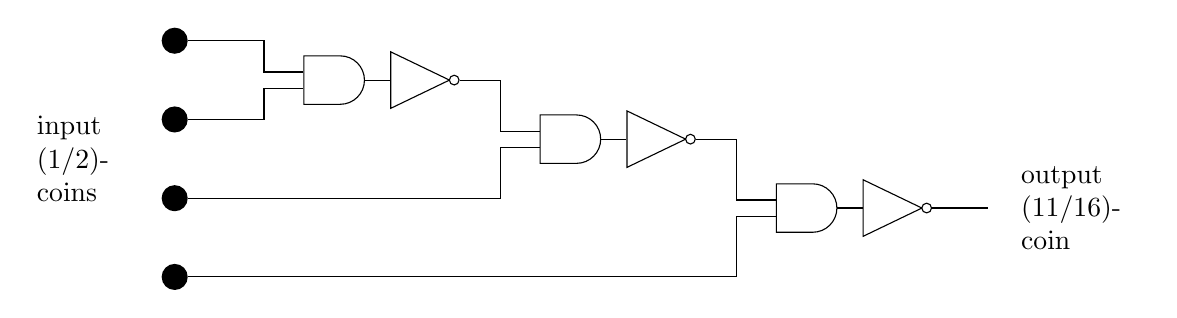
\begin{tikzpicture}[circuit logic US]
\node[circle, fill=black] at (0,0) (coin1) {} ;
\node[circle, fill=black] at (0,-1) (coin2) {} ;
\node[circle, fill=black] at (0,-2) (coin3) {} ;
\node[circle, fill=black] at (0,-3) (coin4) {} ;
\node[circle] at (10.5, -17/8) (output) {} ;

\node[and gate, draw, inputs={nn}] at (2,-1/2) (and1) {} ;
\node[not gate, draw] at (3,-0.5) (not1) {} ;
\node[and gate, draw, inputs={nn}] at (5,-5/4) (and2) {} ;
\node[not gate, draw] at (6,-1.25) (not2) {} ;
\node[and gate, draw, inputs={nn}] at (8, -17/8) (and3) {} ;
\node[not gate, draw] at (9, -17/8) (not3) {} ;

\draw (and1.input 1) -- ++(left:5mm) |- (coin1.east) ;
\draw (and1.input 2) -- ++(left:5mm) |- (coin2.east) ;
\draw (and1.output) -- (not1.input) ;
\draw (and2.input 1) -- ++(left:5mm) |- (not1.output) ;
\draw (and2.input 2) -- ++(left:5mm) |- (coin3.east) ;
\draw (and2.output) -- (not2.input) ;
\draw (and3.input 1) -- ++(left:5mm) |- (not2.output) ;
\draw (and3.input 2) -- ++(left:5mm) |- (coin4.east) ;
\draw (and3.output) -- (not3.input) ;
\draw (not3.output) -- (output) ;

\node[text width = 1.5cm] at (-1,-3/2) (label1) {input (1/2)-coins} ;
\node[text width = 1.5cm] at (11.5,-17/8) (label2) {output (11/16)-coin} ;
\end{tikzpicture}
\end{figure}


\end{proof}


\bibliography{qbf.bib}
\end{document}